\documentclass[a4paper]{article}

\usepackage{amsmath}
\usepackage{amsfonts}
\usepackage{graphicx}
\usepackage{hyperref}
\usepackage[usenames,dvipsnames]{color}

\setlength{\parindent}{0pt}
\setlength{\parskip}{0.75ex plus 0.5ex minus 0.3ex}
\setcounter{secnumdepth}{0} % Do not number sections
\setcounter{tocdepth}{2}

\newcommand{\sympy}{\textbf{\texttt{\textcolor{OliveGreen}{SymPy}} }}

\begin{document}
% ******************************************************************************
\title{Linear Algebra Step by Step in \sympy}

\author{Dario Beraldi}
\maketitle
\tableofcontents

\begin{abstract}
\noindent Excerpts from \textit{Linear Algebra Step by Step} by K. Singh 
with \sympy implementation.
\end{abstract}

% ==============================================================================
\section{1. Linear Equations and Matrices}
% ========================================

\subsection{Solving linear systems}
% ---------------------------------

\subsubsection{Exercises 1.1 2f} 
% ...............................

\begin{equation}\label{eq:ex2f}
    \begin{matrix}
    e x - e y = 2 \\
    e x + e y = 0
    \end{matrix}
\end{equation}

\begin{verbatim}
x, y= symbols('x y', real= true)
eq1= Eq(E*x - E*y, 2)
eq2= Eq(E*x + E*y, 0)
sols= solve([eq1, eq2])
\end{verbatim}

Solved for:

\begin{equation}\label{eq:ex2fsol}
\begin{Bmatrix}x : e^{-1}, & y : - \frac{1}{e}\end{Bmatrix}
\end{equation}

Check solutions by substituting them in the original equations \ref{eq:ex2f}

\begin{verbatim}
eq1.subs(sols)
True
eq2.subs(sols)
True
\end{verbatim}

Solve the system \ref{eq:ex2f} using matrix notation

\begin{verbatim}
coeffs= Matrix([[E, -E], [E, E]])
const= Matrix([2, 0])
[coeffs, const]
\end{verbatim}

\begin{equation}\label{eq:na}
\begin{bmatrix}\left[\begin{matrix}e & - e\\e & e\end{matrix}\right], & \left[\begin{matrix}2\\0\end{matrix}\right]\end{bmatrix}
\end{equation}

If everything is correct, solutions are consistent with \ref{eq:ex2fsol}:

\begin{verbatim}
coeffs.solve(const)
\end{verbatim}

\begin{equation}
\left[\begin{matrix}e^{-1}\\- \frac{1}{e}\end{matrix}\right]
\end{equation}

\subsubsection{Exercises 1.1 4a}
Plot the graphs of these linear equations
% .....................................................

\begin{equation}\label{eq:na}
\begin{matrix}2 x + y = 3\\x - y = 7\end{matrix}
\end{equation}

\begin{verbatim}
eq1= Eq(2*x + y, 3)
eq2= Eq(x - y, 7)
\end{verbatim}

Plot

\begin{verbatim}
pp1= plot_implicit(eq1)
pp2= plot_implicit(eq2)
pp1.extend(pp2)
pp1.save('figs/ex4a.pdf')
\end{verbatim}

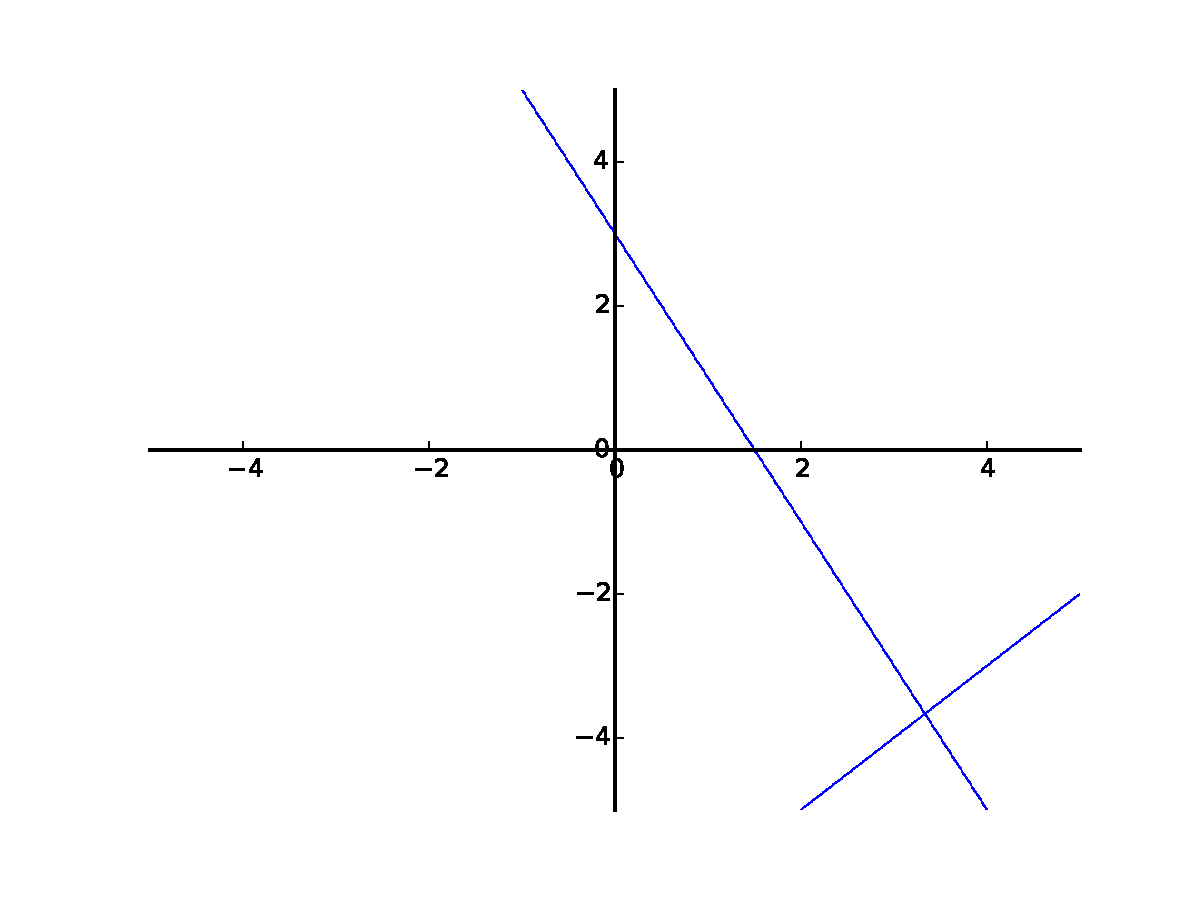
\includegraphics[width=\linewidth]{figs/ex4a.pdf}

\textbf{Exercises 1.1 5b}
% ............

\begin{verbatim}
eq1= Eq(12*x + 4*y, 16)
eq2= Eq(8*x + 4*y, 16)

pp1= plot_implicit(eq1)
pp2= plot_implicit(eq2)
pp1.extend(pp2)
pp1.save('figs/ex5b.pdf')
\end{verbatim}

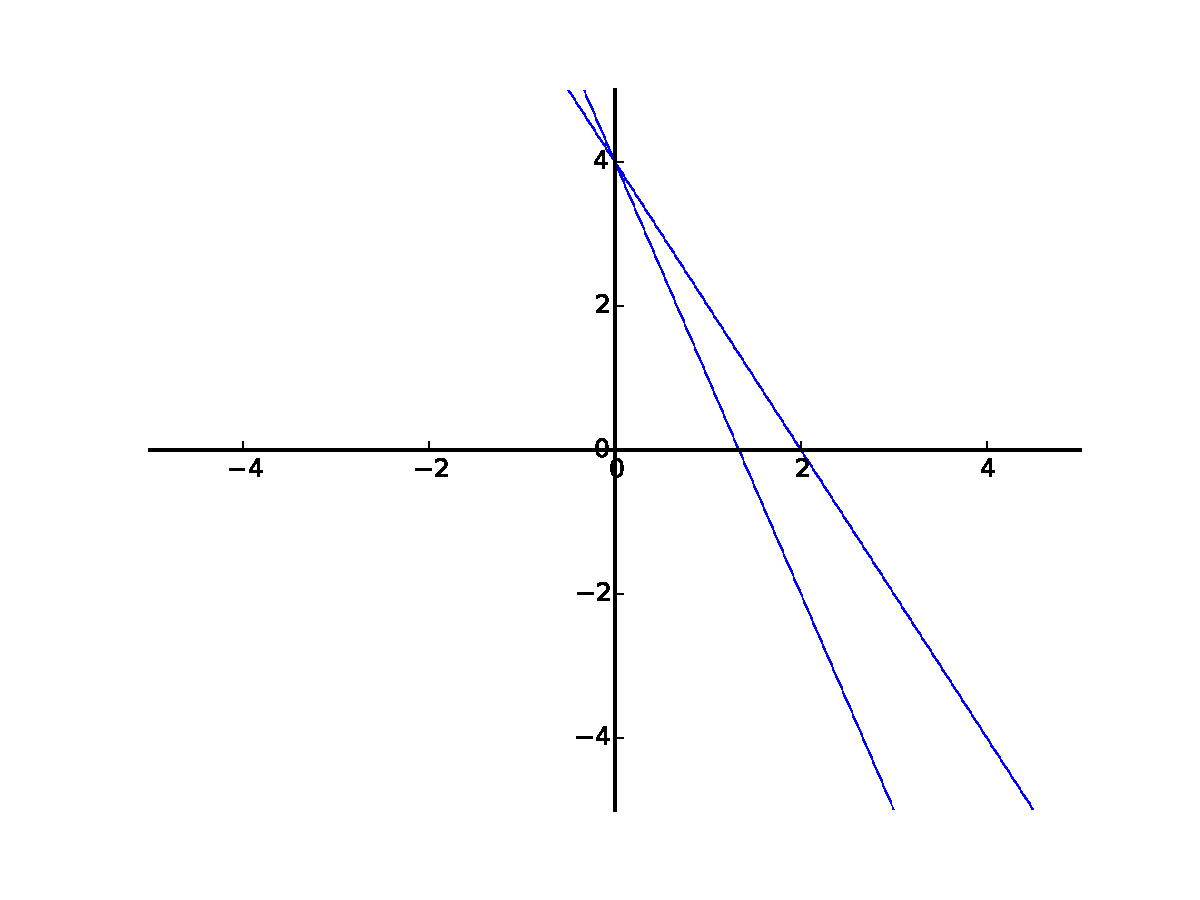
\includegraphics[width=\linewidth]{figs/ex5b.pdf}

\subsection{Solve by row echelon form}
% ------------------------------------

Given a linear system of equations, the solutions can be found by Gaussian
elimination:

\begin{itemize}
\item Extract the coefficients and constants from the equations and put them in
an augmented matrix.
\item Transform the augmented matrix in reduced row echelon form (rref). This is
the result of the Gaussian elimination process.
\item The last columns of the rref matrix lists the solutions of the linear system.
\end{itemize}

Reminder: rref means that every leading coefficient is 1 and is the only nonzero
entry in its column \footnote{http://en.wikipedia.org/wiki/Row\_echelon\_form}. 

\subsubsection{Exercises 1.2 2a}

\begin{equation}\label{eq:na}
\begin{matrix}x + 2 y + 3 z = 12\\2 x - y + 5 z = 3\\3 x + 3 y + 6 z = 21\end{matrix}
\end{equation}

\begin{verbatim}
eq1= Eq(x + 2*y + 3*z, 12)
eq2= Eq(2*x - y + 5*z, 3)
eq3= Eq(3*x + 3*y + 6*z, 21)
\end{verbatim}

Represent the linear systen as \textit{augmented} matrix, where the last column
holds the constants:

\begin{equation}\label{eq:na}
M= \left[\begin{matrix}1 & 2 & 3 & \textit{12}\\
                       2 & -1 & 5 & \textit{3}\\
                       3 & 3 & 6 & \textit{21}\end{matrix}\right]
\end{equation}

In \sympy use the \href{http://docs.sympy.org/latest/modules/polys/reference.html#sympy.polys.polytools.Poly}{\texttt{Poly}}
class to conveniently extract the coefficients at the left hand side of
the equations:

\begin{verbatim}
M= Matrix([
    Poly(eq1.lhs).coeffs(),
    Poly(eq2.lhs).coeffs(),
    Poly(eq3.lhs).coeffs()
])
const= Matrix([eq1.rhs, eq2.rhs, eq3.rhs])
M= const.col_insert(0, M)
\end{verbatim}

In reduced row echelon form, with indexes of the pivot variables on the right:

\begin{equation}\label{eq:na}
RREF= \begin{pmatrix}\left[\begin{matrix}1 & 0 & 0 & 1\\0 & 1 & 0 & 4\\0 & 0 & 1 & 1\end{matrix}\right], & \begin{bmatrix}0, & 1, & 2\end{bmatrix}\end{pmatrix}
\end{equation}

Solutions can be read from last column of the RREF $\left[\begin{matrix}x:1\\y:4\\z:1\end{matrix}\right]$. Verify the solutions solve
the initial system of equations:

\begin{verbatim}
rref= M.rref()
sols= rref[0].col(-1)

eq1.subs({x:sols[0], y:sols[1], z:sols[2]}) # True
eq2.subs({x:sols[0], y:sols[1], z:sols[2]}) # True
eq3.subs({x:sols[0], y:sols[1], z:sols[2]}) # True

# Or the same returning dict {x: 1, y: 4, z: 1}
solve([eq1, eq2, eq3]) 
\end{verbatim}

\subsubsection{Exercises 1.2 3d}
% ..............................

Linear system:

\begin{equation}\label{eq:na}
\begin{matrix}
    - 2 x + 3 y - 2 z = 8 \\
    - x + 2 y - 10 z = 0 \\
    5 x - 7 y + 4 z = -20
\end{matrix}
\end{equation}

Augmented matrix:

\begin{equation}\label{eq:na}
\left[\begin{matrix}-2 & 3 & -2 & 8\\-1 & 2 & -10 & 0\\5 & -7 & 4 & -20\end{matrix}\right]
\end{equation}

Reduced row echelon form with solutions in the last column:

\begin{equation}\label{eq:na}
\begin{pmatrix}\left[\begin{matrix}1 & 0 & 0 & -3 \\
                                   0 & 1 & 0 & 1 \\
                                   0 & 0 & 1 &
\frac{1}{2}\end{matrix}\right], & \begin{bmatrix}0, & 1, & 2\end{bmatrix}\end{pmatrix}
\end{equation}

In \sympy:

\begin{verbatim}
eq1= Eq(-2*x + 3*y -2*z, 8)
eq2= Eq(-x + 2*y - 10*z, 0)
eq3= Eq(5*x - 7*y + 4*z, -20)

M= Matrix([
    Poly(eq1.lhs).coeffs(),
    Poly(eq2.lhs).coeffs(),
    Poly(eq3.lhs).coeffs()
])
const= Matrix([eq1.rhs, eq2.rhs, eq3.rhs])
M= const.col_insert(0, M)
rref= M.rref()
sols= rref[0].col(-1)

# Checked: {x: -3, y: 1, z: 1/2}
solve([eq1, eq2, eq3])
\end{verbatim}

\subsection{Vector arithmetic}
% ----------------------------

\subsubsection{Exercise 1.3.1}

Given two vectors:

\begin{verbatim}
va= Matrix([2, 0])
vb= Matrix([2, 1])
\end{verbatim}

plot the results of the operations 

\subsubsection{(a-e)}

\begin{verbatim}
vA= va + vb          # [4 1]
vB= va - vb          # [0 -1]
vC= 3 * va           # [6 0]
vD= -1/2 * vb        # [-1 -0.5]
vE= 3*va - 1/2 * vb  # [5 -0.5]
\end{verbatim}

And plot vectors

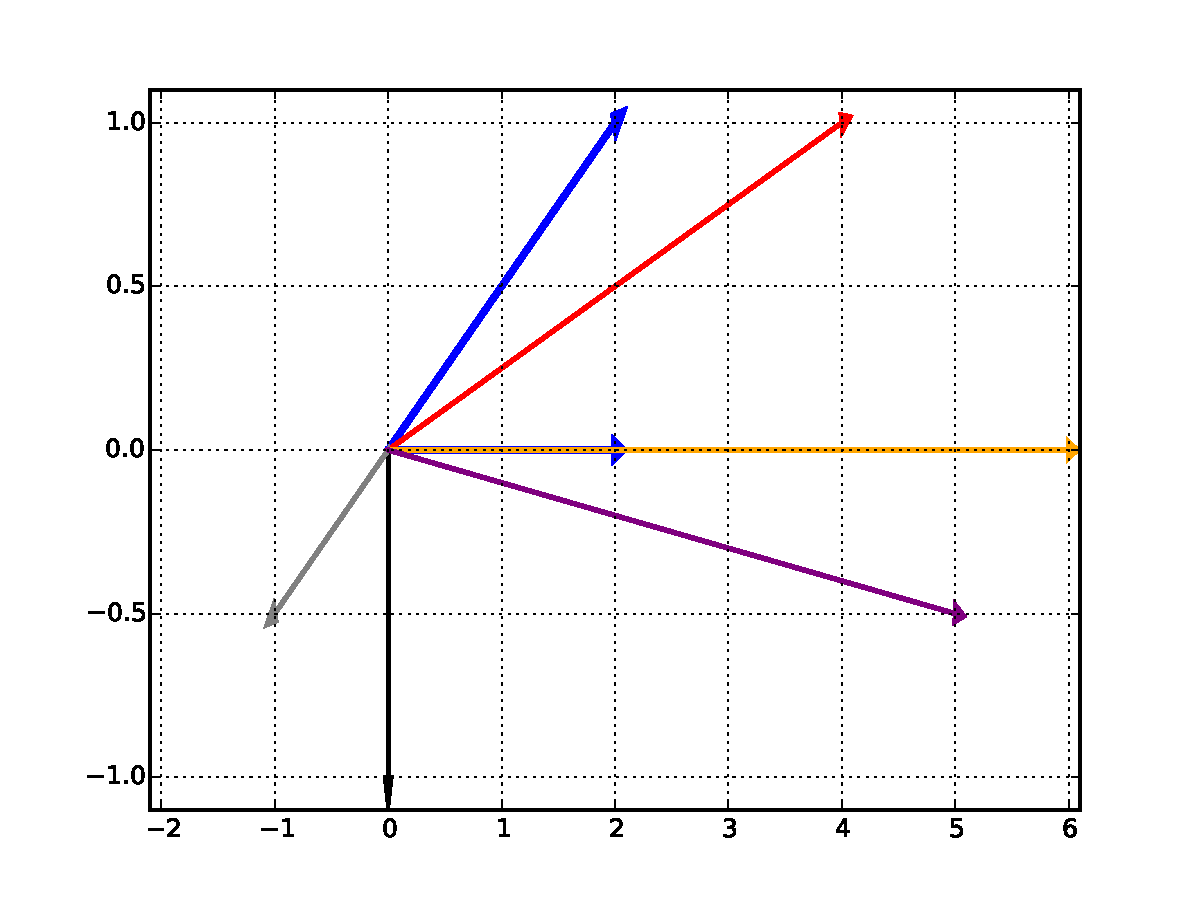
\includegraphics[width=\linewidth]{figs/ex1_3.pdf}

\begin{verbatim}
plt.arrow(0, 0, float(va[0]), float(va[1]), lw= 3, color= 'b', head_width=0.05)
plt.arrow(0, 0, float(vb[0]), float(vb[1]), lw= 3, color= 'b', head_width=0.05)
plt.arrow(0, 0, float(vA[0]), float(vA[1]), lw= 2, color= 'r', head_width=0.05)
plt.arrow(0, 0, float(vB[0]), float(vB[1]), lw= 2, color= 'black', head_width=0.05)
plt.arrow(0, 0, float(vC[0]), float(vC[1]), lw= 2, color= 'orange', head_width=0.05)
plt.arrow(0, 0, float(vD[0]), float(vD[1]), lw= 2, color= 'grey', head_width=0.05)
plt.arrow(0, 0, float(vE[0]), float(vE[1]), lw= 2, color= 'purple', head_width=0.05)
plt.xlim(-2.1, 6.1)
plt.ylim(-1.1, 1.1)
plt.grid()
plt.savefig('figs/ex1_3.pdf')
plt.close()
\end{verbatim}

\subsubsection{Exercise 1.3.8}
% ............................
Show that $x\mathbf{u} + y\mathbf{v} = \mathbf{w}$ where
$\mathbf{u}= (1\ 0)^{T}$, $\mathbf{v}= (0\ 1)^{T}$, and $\mathbf{w}= (x\ y)^{T}$.

This is a consequence of $x(1\ 0) = (x\ 0)$ and $y(0\ 1) = (y\ 0)$. So that
$(x\ 0) + (0\ y) = (x\ y)$

\begin{verbatim}
x, y= symbols('x y')
u= Matrix([1, 0])
v= Matrix([0, 1])
w= Matrix([x, y])
Eq(x*u + y*v, w) # True
\end{verbatim}

\subsubsection{Exercise 1.3.12}
% .............................

Find the real numbers x, y and z, if

\begin{equation}\label{eq:na}
\left[\begin{matrix}x - 2 z\\2 x + y\\- y + 6 z\end{matrix}\right] = \left[\begin{matrix}5\\3\\17\end{matrix}\right]
\end{equation}

Which is solved for:

\begin{equation}\label{eq:}
sols= \begin{bmatrix}\begin{Bmatrix}x : 7, & y : -11, & z : 1\end{Bmatrix}\end{bmatrix}
\end{equation}

\begin{verbatim}
eq1= Eq(x * Matrix([1, 2, 0]) + y * Matrix([0, 1, -1]) + z * Matrix([-2, 0, 6]),
    Matrix([5, 3, 17]))
sols= solve(eq1)
\end{verbatim}

\subsubsection{Exercise 1.3.12}
% .............................

Show that vectors \textbf{u} and \textbf{v} in space $\mathbb{R}^n$ can be
$\mathbf{u} \cdot{} \mathbf{v} = \mathbf{0}$ even if neither \textbf{u} or \textbf{v}
are 0 vectors.

Set:

\begin{verbatim}
u= Matrix([-1, 1])
v= Matrix([1, 1])
u.dot(v) == 0 # True
\end{verbatim}

\subsection{Arithmetic of Matrices}
% ---------------------------------

\subsubsection{Exercise 1.4.1}
% .............................

Given matrix \textbf{B}, note that $3\mathbf{B} = \mathbf{B} + \mathbf{B} + \mathbf{B}$

\begin{equation}
\left[\begin{matrix}6 & -1\\5 & 3\end{matrix}\right]
\end{equation}

\begin{verbatim}
B= Matrix([[6, -1], [5, 3]])
3*B == (B + B + B)
\end{verbatim}

\subsubsection{Exercise 1.4.6}
% .............................

Note how matrx multiplication can result in zero matrix:

\begin{equation}
\left[\begin{matrix}5 & -1 & -2\\10 & -2 & -4\\15 & -3 & -6\end{matrix}\right]
\left[\begin{matrix}1 & 1 & 3\\1 & -1 & -1\\2 & 3 & 8\end{matrix}\right]
= \left[\begin{matrix}0 & 0 & 0\\0 & 0 & 0\\0 & 0 & 0\end{matrix}\right]
\end{equation}

\begin{verbatim}
A= Matrix(3, 3, [5, -1, -2, 10, -2, -4, 15, -3, -6])
B= Matrix(3, 3, [1, 1, 3, 1, -1, -1, 2, 3, 8])
Z= A * B
\end{verbatim}

\subsubsection{Exercise 1.4.8}
% ............................

$\mathbf{x}_n = \mathbf{A}^n\mathbf{x}$ Describes a \textbf{discrete dynamical
system}. Apply this formula to

\begin{equation}\label{eq:ex148}
A = \left[\begin{matrix}0.5 & 0.5\\0.5 & 0.5\end{matrix}\right]
\end{equation}

\begin{verbatim}
A= Matrix(2, 2, [1/2, 1/2, 1/2, 1/2])
\end{verbatim}

For the matrix in \ref{eq:ex148} $A^n = A$:

\begin{verbatim}
A**2 == A # True
A**3 == A # True
A**10 == A # True
\end{verbatim}

matrix in \ref{eq:ex148} is a Markov matrix since the colum sums equal 1.

\subsubsection{Exercise 1.4.10}
% .............................

Determine the image of the matrix \textbf{F} after transformation \textbf{AF}:

\begin{equation}
A = \left[\begin{matrix}1 & 0.2\\0 & 1\end{matrix}\right]
\end{equation}

\begin{equation}
F = \left[\begin{matrix}1 & 1 & 2 & 2 & 1.4 & 1.4 & 2 & 2 & 1.4 & 1.4\\1 & 3 & 3 & 2.6 & 2.6 & 2 & 2 & 1.6 & 1.6 & 1\end{matrix}\right]
\end{equation}

\begin{equation}\label{eq:}
AF = \left[\begin{matrix}1.2 & 1.6 & 2.6 & 2.52 & 1.92 & 1.8 & 2.4 & 2.32 & 1.72 & 1.6\\1 & 3 & 3 & 2.6 & 2.6 & 2 & 2 & 1.6 & 1.6 & 1\end{matrix}\right]
\end{equation}

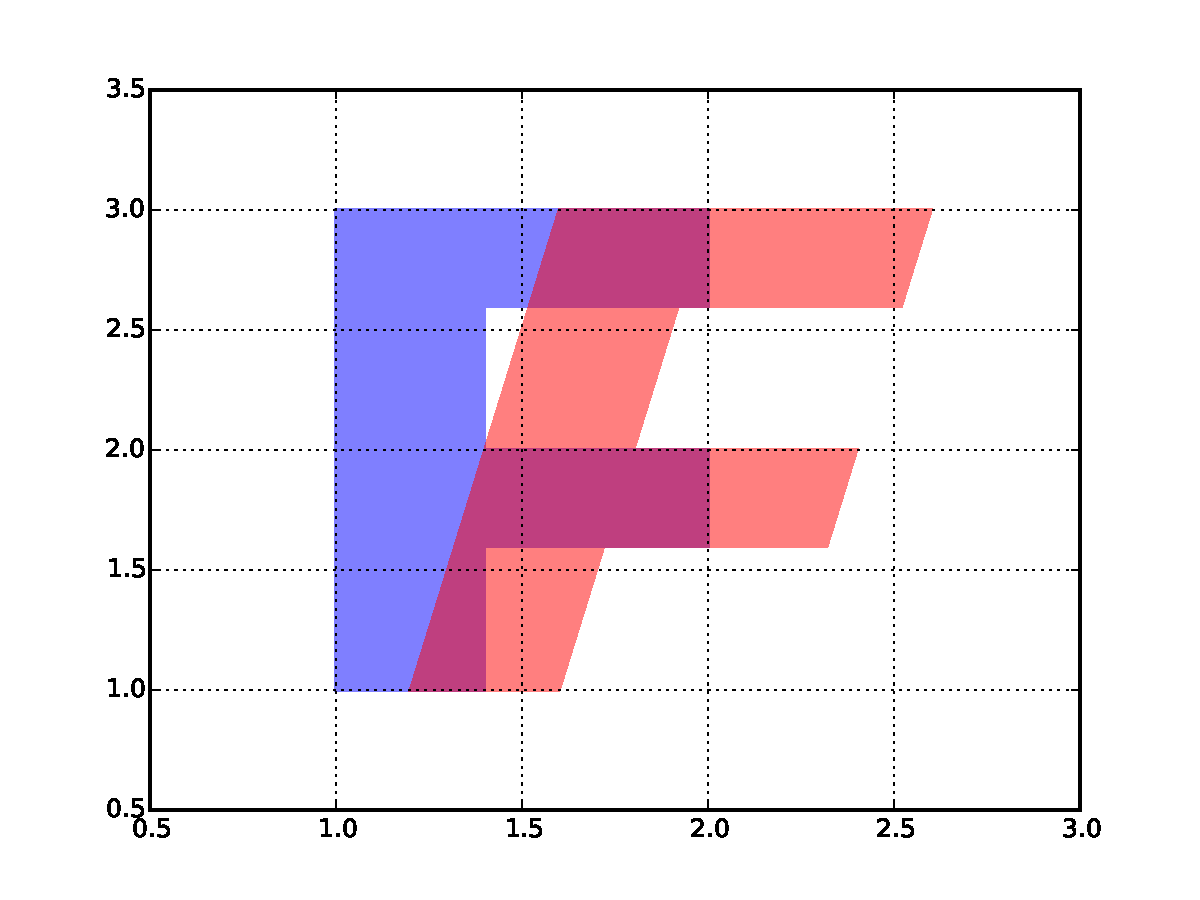
\includegraphics[width=\linewidth]{figs/1_4_10.pdf}

This is showing that the matrix operation $\mathbf{AF} = \mathbf{F_2}$ can be seen as
$\mathbf{f(F)}= \mathbf{F_2}$. That is, the matrix on the left-hand (\textbf{A})
side acts like a function that transforms its argument (\textbf{F}).

\begin{verbatim}
A= Matrix([[1, 0.2], [0, 1]])
F= Matrix([
    [1, 1, 2, 2, 1.4, 1.4, 2, 2, 1.4, 1.4],
    [1, 3, 3, 2.6, 2.6, 2, 2, 1.6, 1.6, 1]])

AF= A*F

verts_F= []
for i in range(F.cols):
    verts_F.append((F[0, i], F[1, i]))
verts_AF= []
for i in range(AF.cols):
    verts_AF.append((AF[0, i], AF[1, i]))

fig = plt.figure()
ax = fig.add_subplot(1, 1, 1)
poly_F = patches.Polygon(verts_F, color= 'b', alpha= 0.5)
poly_AF = patches.Polygon(verts_AF, color= 'r', alpha= 0.5)
ax.set_xlim((0.5, 3))
ax.set_ylim((0.5, 3.5))
ax.add_patch(poly_F)
ax.add_patch(poly_AF)
plt.grid()
plt.savefig('figs/1_4_10.pdf')
\end{verbatim}

\subsubsection{Exercise 1.4.11}
% .............................

\begin{verbatim}
O= Matrix.zeros(2, 1)
X= Matrix([x, y])
\end{verbatim}

\begin{verbatim}
A= Matrix([[1, 2], [3, 5]])
xy= A.solve(O) # x:0, y:0
# Or
xy= A.LUsolve(O) 
# Or
solve(A*X)

A= Matrix([[2, 7], [3, 15]]) # x:0, y:0
xy= A.solve(O)

A= Matrix([[1, 4], [3, 12]]) # Linearly dependent!
xy= A.solve(O)
>>> ValueError: Matrix det == 0; not invertible.
\end{verbatim}

\subsubsection{Exercise 1.4.12}
% .............................

Determine whether vector \textbf{w} is a linear combination of vector \textbf{u}
and \textbf{v}.

Effectively this is asking if the equation $x\mathbf{u} + y\mathbf{v} = \mathbf{w}$
can be resolved.


\begin{itemize}
\item Create an augmented matrix as [u, v, w].
\item Transform the augmented matrix in row echelon form.
\item Get coefficients x and y from last column of RREF. The three vectors are linearly
independent and \textbf{w} $\neq$ \textbf{u} + \textbf{v} (\textbf{w} is not a linear
combination of \textbf{u} and \textbf{v}).

\end{itemize}

\begin{verbatim}
w= Matrix(2, 1, [1, 0])
u= Matrix(2, 1, [5, 8])
v= Matrix(2, 1, [2, 4])
A=  w.col_insert(0, v).col_insert(0, u)
A.rref()
\end{verbatim}

\begin{equation}
REF= \begin{pmatrix}\left[\begin{matrix}1 & 0 & 1\\0 & 1 & -2\end{matrix}\right], & \begin{bmatrix}0, & 1\end{bmatrix}\end{pmatrix}
\end{equation}

\textbf{w} is a linear combination. In fact $1\mathbf{u} -2\mathbf{v}= \mathbf{w}$

\begin{verbatim}
w= Matrix(2, 1, [0, 1])
u= Matrix(2, 1, [5, 8])
v= Matrix(2, 1, [2, 4])
A=  w.col_insert(0, v).col_insert(0, u)
A.rref()
\end{verbatim}

\begin{equation}\label{eq:}
\begin{pmatrix}\left[\begin{matrix}1 & 0 & - \frac{1}{2}\\0 & 1 & \frac{5}{4}\end{matrix}\right], & \begin{bmatrix}0, & 1\end{bmatrix}\end{pmatrix}
\end{equation}

\begin{verbatim}
w= Matrix(3, 1, [1, 2, 3])
u= Matrix(3, 1, [1, 0, 0])
v= Matrix(3, 1, [0, 1, 0])
A=  w.col_insert(0, v).col_insert(0, u)
A.rref()
\end{verbatim}

\begin{equation}
REF= \begin{pmatrix}\left[\begin{matrix}1 & 0 & 0\\0 & 1 & 0\\0 & 0 & 1\end{matrix}\right], & \begin{bmatrix}0, & 1, & 2\end{bmatrix}\end{pmatrix}
\end{equation}

\textbf{w} cannot be a linear combination. In fact
$0\mathbf{u} + 0\mathbf{v} \neq [1\ 2\ 3]^T$

\begin{verbatim}
w= Matrix(3, 1, [1, 2, 3])
u= Matrix(3, 1, [4, 8, 0])
v= Matrix(3, 1, [1, 2, -3/7])
A=  w.col_insert(0, v).col_insert(0, u)
A.rref()
\end{verbatim}

\begin{equation}\label{eq:}
\begin{pmatrix}\left[\begin{matrix}1 & 0 & 2.0\\0 & 1.0 & -7.0\\0 & 0 & 0\end{matrix}\right], & \begin{bmatrix}0, & 1\end{bmatrix}\end{pmatrix}
\end{equation}

\subsection{Matrix Algebra}
% -------------------------

\subsubsection{Exrcises 1.5.2}
% ............................

Given $A = \left[\begin{matrix}5 & -1 & -2\\1 & -3 & 2\end{matrix}\right]$

A) Find \textbf{B} suc that \textbf{A} + \textbf{B} = \textbf{O} with \textbf{O}
a 2 x 3 matrix.

Requires $\mathbf{A} = \mathbf{B} \Rightarrow \mathbf{B} = -\mathbf{A}$

\begin{verbatim}
A= Matrix([[5, -1, -2], [1, -3, 2]])
O= Matrix.zeros(2, 3)
\end{verbatim}


\subsubsection{Exrcises 1.5.7}
% ----------------------------

Determine the scalar $\lambda$ so that $\mathbf{Ax} = \lambda \mathbf{x}$ with
$\mathbf{A} = \left[\begin{matrix}2 & 1 \\ 1 & 2\end{matrix}\right]$ and $\mathbf{x} = \left[\begin{matrix} 1\\1 \end{matrix}\right]$

$\lambda = 3$ since $\mathbf{Ax} = [3\ 3]^T$.

\begin{verbatim}
A= Matrix([[2, 1], [1, 2]])
x= Matrix(2, 1, [1, 1])
l= symbols('lambda')
solve(Eq(A*x, l*x)) # Lambda= 3
\end{verbatim}

\subsubsection{Exrcises 1.5.10}
% ----------------------------

Given \textbf{T} a transition matrix from a Markov chain and \textbf{p} a
probability vector. Note that the probility vector must sum to 1.

What is the probility that the chain is in a given state after $k$ steps?

The answer is given by $\mathbf{p}_k = \mathbf{T}^k\mathbf{p}$.

For:
\begin{equation}
\left[\begin{matrix}0.6 & 0.7\\0.4 & 0.3\end{matrix}\right]
\end{equation}

\begin{equation}
\left[\begin{matrix}0.5\\0.5\end{matrix}\right]
\end{equation}

Determine $\mathbf{p}_k$ for $k$ in 1, 2, 10, 100, 100000:

$p_{k= 1} = \left[\begin{matrix}0.65\\0.35\end{matrix}\right]$

$p_{k= 2} = \left[\begin{matrix}0.635\\0.365\end{matrix}\right]$

$p_{k= 10} = \left[\begin{matrix}0.63636363635\\0.36363636365\end{matrix}\right]$

$p_{k= 100} = \left[\begin{matrix}0.636363636363634\\0.363636363636362\end{matrix}\right]$

$p_{k= 100000} = \left[\begin{matrix}0.636363636361267\\0.36363636363501\end{matrix}\right]$

Note how the probability vector converges in the long period. The probability vector
at the initial state $k = 0$ might represent the proportion of different species
in the environment. Given the probility of change in \textbf{T}, we can ask the question:
What proportion of species we will see after $k$ iterations (\textit{e.g} generations)?

\begin{verbatim}
T= Matrix(2,2, [0.6, 0.7, 0.4, 0.3])
p= Matrix(2, 1, [0.5, 0.5])
ks= [1, 2, 10, 100, 100000]

for k in ks:
    p_k= T**k * p
    print latex(p_k)
\end{verbatim}


\subsection{Type of solutions}
% ========================================

\subsubsection{Exrcises 1.7.8}
% ----------------------------

\begin{equation}\label{eq:}
\textbf{M} = \left[\begin{matrix}1 & 1 & 1 & 0 & 0 & 0 & 6\\0 & 0 & 0 & 1 & 1 & 1 & 15\\1 & 0 & 0 & 1 & 0 & 0 & 5\\0 & 1 & 0 & 0 & 1 & 0 & 7\\0 & 0 & 1 & 0 & 0 & 1 & 9\end{matrix}\right]
\end{equation}

\begin{equation}\label{eq:}
\mathbf{M_{rref}}= \begin{pmatrix}\left[\begin{matrix}1 & 0 & 0 & 0 & -1 & -1 & -10\\0 & 1 & 0 & 0 & 1 & 0 & 7\\0 & 0 & 1 & 0 & 0 & 1 & 9\\0 & 0 & 0 & 1 & 1 & 1 & 15\\0 & 0 & 0 & 0 & 0 & 0 & 0\end{matrix}\right], & \begin{bmatrix}0, & 1, & 2, & 3\end{bmatrix}\end{pmatrix}
\end{equation}

There are six variables with coefficents arranged as in matrix $\mathbf{M}$. In
RREF it appears the first four variables, $x_1$ to $x_4$, have 1 as leading
coefficient, as reported by \sympy in the list of pivot variables indexes on the right
(0, 1, 2, 3). Variables $x_5$ and $x_6$ are \textit{free} with coefficients given
in the respective columns. The solutions are therefore:

\begin{equation}\label{eq:}
\begin{Bmatrix}x_{1} : x_{5} + x_{6} - 10, & x_{2} : - x_{5} + 7, & x_{3} : - x_{6} + 9, & x_{4} : - x_{5} - x_{6} + 15\end{Bmatrix}
\end{equation}

\begin{verbatim}
M= Matrix([
[1, 1, 1, 0, 0, 0, 6],
[0, 0, 0, 1, 1, 1, 15],
[1, 0, 0, 1, 0, 0, 5],
[0, 1, 0, 0, 1, 0, 7],
[0, 0, 1, 0, 0, 1, 9],
])
M_rref= M.rref()
\end{verbatim}

Solve system of equations:

\begin{verbatim}
x1, x2, x3, x4, x5, x6= symbols('x1:7')
r1= Eq(x1 + x2 + x3, 6)
r2= Eq(x4 + x5 + x6, 15)
r3= Eq(x1 + x4, 5)
c1= Eq(x2 + x5, 7)
c2= Eq(x3 + x6, 9)
sols= solve([r1, r2, r3, c1, c2])
\end{verbatim}

\subsubsection{Exrcises 1.7.11}
% ----------------------------

\begin{verbatim}
x, y, z, t= symbols('x y z t', real= True)

eq1= Eq(2*x - 4*y + 4*z + 0.077*t, 3.86)
eq2= Eq(     -2*y + 2*z - 0.056*t, -3.47)
eq3= Eq(2*x - 2*y,                 0)
sols= solve([eq1, eq2, eq3], [x, y, z])
\end{verbatim}

The solutions \texttt{sols}  are in \ref{eq:ex1_7_11}.

Solving via augmented matrix in reduced row echelon form:

\begin{verbatim}
M= Matrix([
    [2, -4, 4, 0.077, 3.86],
    [0, -2, 2, -0.056, -3.47],
    [2, -2, 0, 0, 0]
])
M_rref= M.rref()
\end{verbatim}

\begin{equation}\label{eq:}
\begin{matrix}
2 x - 4 y + 4 z + 0.077 t= 3.86, & \\
- 2 y + 2 z - 0.056 t = -3.47, & \\
2 x - 2 y = 0\end{matrix}
\end{equation}

\begin{equation}\label{eq:}
M= \left[\begin{matrix}2 & -4 & 4 & 0.077 & 3.86\\0 & -2 & 2 & -0.056 & -3.47\\2 & -2 & 0 & 0 & 0\end{matrix}\right]
\end{equation}

\begin{equation}\label{eq:}
M_{rref} = \begin{pmatrix}\left[\begin{matrix}1 & 0 & 0 & 0.0945 & 5.4\\0 & 1 & 0 & 0.0945 & 5.4\\0 & 0 & 1 & 0.0665 & 3.665\end{matrix}\right], & \begin{bmatrix}0, & 1, & 2\end{bmatrix}\end{pmatrix}
\end{equation}

Note that the 4th column holds the coefficients for the free variable $t$ while the
last column has the values for $x, y, z$. Compare to the solutions
from \sympy \texttt{solve}:

\begin{equation}\label{eq:ex1_7_11}
\begin{Bmatrix}x : - 0.0945 t + 5.4, & y : - 0.0945 t + 5.4, & z : - 0.0665 t + 3.665\end{Bmatrix}
\end{equation}

\subsection{The inverse matrix method}
% ====================================

\subsubsection{Exrcises 1.8.3}
% ----------------------------

What effect has the matrix \textbf{E} on the matrix \textbf{A}. With \textbf{A}
a generic 3x3 matrix:

\begin{verbatim}
x1, x2, x3, x4, x5, x6, x7, x8, x9= symbols('x1:10')
k= symbols('k', zero= False)
A= Matrix(3,3, [x1, x2, x3, x4, x5, x6, x7, x8, x9])
\end{verbatim}

\begin{equation}\label{eq:1_8_3A}
\mathbf{A} = \left[\begin{matrix}x_{1} & x_{2} & x_{3}\\x_{4} & x_{5} & x_{6}\\x_{7} & x_{8} & x_{9}\end{matrix}\right]
\end{equation}

\begin{equation}\label{eq:}
\mathbf{E} = \left[\begin{matrix}1 & 0 & 0\\0 & -1 & 0\\0 & 0 & 1\end{matrix}\right]
\end{equation}

\begin{verbatim}
E_a= Matrix([
    [1, 0, 0],
    [0, -1, 0],
    [0, 0, 1]
])
print latex(E_a * A)
\end{verbatim}

\begin{equation}\label{eq:}
\mathbf{E_aA} = \left[\begin{matrix}x_{1} & x_{2} & x_{3}\\- x_{4} & - x_{5} & - x_{6}\\x_{7} & x_{8} & x_{9}\end{matrix}\right]
\end{equation}

\begin{verbatim}
E_b= Matrix([
    [0, 0, 1],
    [0, 1, 0],
    [1, 0, 0]
])
print latex(E_b * A)
\end{verbatim}

\begin{equation}\label{eq:}
\mathbf{E_bA} = \left[\begin{matrix}x_{7} & x_{8} & x_{9}\\x_{4} & x_{5} & x_{6}\\x_{1} & x_{2} & x_{3}\end{matrix}\right]
\end{equation}

\begin{verbatim}
E_c= Matrix([
    [k, 0, 0],
    [0, 1, 0],
    [0, 0, 1]
])
print latex(E_c * A)
\end{verbatim}

\begin{equation}\label{eq:}
\mathbf{E_cA} = \left[\begin{matrix}k x_{1} & k x_{2} & k x_{3}\\x_{4} & x_{5} & x_{6}\\x_{7} & x_{8} & x_{9}\end{matrix}\right]
\end{equation}


\begin{verbatim}
E_d= Matrix([
    [1, 0, 0],
    [0, 1, 0],
    [0, 0, -1/k]
])
print latex(E_d * A)
\end{verbatim}

\begin{equation}\label{eq:}
\mathbf{E_dA} = \left[\begin{matrix}x_{1} & x_{2} & x_{3}\\x_{4} & x_{5} & x_{6}\\- \frac{x_{7}}{k} & - \frac{x_{8}}{k} & - \frac{x_{9}}{k}\end{matrix}\right]
\end{equation}

\subsubsection{Exrcises 1.8.5}
% ----------------------------

Solve the linear systems using inverse matrix method.

\begin{equation}\label{eq:eqs_1_8_5}
\begin{matrix}x + 2 y = 3, & \\ - x + 4 y = 5\end{matrix}
\end{equation}

The coefficients on the LHS of the equations can be thought as a matrix
\textbf{A}. \textbf{A} transforms the vector of unknown coefficients \textbf{x}
to produce the vector of constants \textbf{b} on the RHS:

\begin{equation}\label{eq:1_8_5}
\mathbf{A}\mathbf{x} = \mathbf{b}
\end{equation}

To find the vector \textbf{x} we can rearrange \ref{eq:eqs_1_8_5} as:

\begin{equation}
\mathbf{x} = \mathbf{A}^{-1}\mathbf{b}
\end{equation}

In case of \ref{eq:eqs_1_8_5} we have $\mathbf{A} = \left[\begin{matrix}1 & 2\\-1 & 4\end{matrix}\right]$,
$\mathbf{b} = \left[\begin{matrix}3\\5\end{matrix}\right]$. So
$\mathbf{A^{-1}} = \left[\begin{matrix}\frac{2}{3} & - \frac{1}{3}\\\frac{1}{6} & \frac{1}{6}\end{matrix}\right]$
and $\mathbf{x} = \mathbf{A^{-1}b} = \left[\begin{matrix}\frac{1}{3}\\\frac{4}{3}\end{matrix}\right]$

\begin{verbatim}
x, y= symbols('x y')
eq1= Eq(x + 2*y, 3)
eq2= Eq(-x + 4*y, 5)

A = Matrix(2, 2, [1, 2, -1, 4])
b = Matrix(2, 1, [3, 5])
Ai= A.inv()
x= Ai * b
\end{verbatim}

In case of $\mathbf{Ax = b}$ as:

\begin{equation}\label{eq:}
\left[\begin{matrix}1 & 0 & 2\\2 & 3 & 1\\3 & 6 & 0\end{matrix}\right]
\mathbf{x} = 
\left[\begin{matrix}-1\\1\\9\end{matrix}\right]
\end{equation}

Matrix \textbf{A} is not invertible and the system has no solutions.

\begin{verbatim}
A = Matrix([
[1, 0, 2],
[2, 3, 1],
[3, 6, 0]
])
b= Matrix(3, 1,  [-1 , 1, 9])

Ai= A.inv()
# ValueError: Matrix det == 0; not invertible.
\end{verbatim}

\subsubsection{Exrcises 1.8.7}
% ----------------------------

\textbf{Leontief input-output model}. Represents the production \textbf{p} and
demand \textbf{d} as a matrix. \textbf{p} and \textbf{d} are vectors where each entry
represents a good. The production of goods is represented as a matrix where each row
states how much units of the other goods (input) is required to produce one unit
of that good (output). With this model we can ask how much input is needed to produce
a given amount of output.

$$
\bordermatrix{\text{}& O & E & S \cr
                 O & 0.25 &  0.15  & 0.1 \cr
                 E & 0.4  &  0.15  & 0.2 \cr
                 S & 0.15 &  0.2   & 0.2} = \mathbf{A}
$$

Reading this matrix row by row, it tells how much Oil, Energy and Services it is
needed to produce one unit of O, E, or S. For example 1 unit of O requires 0.25 units
of O, 0.15 of E and 0.1 units of S.

From this matrix we can relate the production vector \textbf{p} to the demand
vector \textbf{d} as:

\begin{equation}\label{eq:1_8_7io}
\mathbf{p} = \mathbf{Ap} + \mathbf{d}
\end{equation}


We want to know \textbf{p} given \textbf{A} and the demand vector \textbf{d}.
\emph{I.e.} we want to solve \ref{eq:1_8_7io} \emph{w.r.t.} \textbf{p} by re-arranging
to the form \textbf{Ax = b}.

$$\mathbf{
p - Ap = d
}$$

then use the identity matrix to obtain the solvable form \textbf{Ax = b}:

$$\mathbf{
p(I - A) = d
}$$

Now solve by inverting \textbf{(I - A)}:

$$\mathbf{
p = (I - A)^{-1} d
}$$

If the demand for O, E, and S is $\mathbf{d} = [100, 100, 100]^T$ we need to
produce
$\left[\begin{matrix}O \\ E \\ S \end{matrix}\right] = \left[\begin{matrix}220 \\ 276 \\ 235 \end{matrix}\right]$

\begin{verbatim}
A = Matrix([
[0.25, 0.15, 0.1],
[0.4, 0.15, 0.2],
[0.15, 0.2, 0.2]
])

d= Matrix(3, 1, [100, 100, 100])
ii= eye(A.rows)
p= (ii - A).inv() * d
\end{verbatim}



\subsubsection{Exrcises 1.8.8}
% ----------------------------

Show that if \textbf{A} is invertible then $A^Tx=b$ has a unique solution.

\begin{verbatim}
x1, x2, x3, x4, x5, x6, x7, x8, x9= symbols('x1:10')
A= Matrix(3,3, [x1, x2, x3, x4, x5, x6, x7, x8, x9])

k1, k2, k3= symbols('k1:4')
b= Matrix(3, 1, [k1, k2, k3])

A_rref= A.transpose().solve(b).rref()
\end{verbatim}

\begin{equation}\label{eq:}
\mathbf{A_{rref}} = \begin{pmatrix}\left[\begin{matrix}1\\0\\0\end{matrix}\right], & \begin{bmatrix}0\end{bmatrix}\end{pmatrix}
\end{equation}

\textit{Does it mean there is a unique solution?}
\section{2. Euclidean Space}
% **************************

\subsection{Properties of vectors}
% ================================

Dot product, norm and distances. The dot product of two vectors \textbf{A} and
\textbf{B} can be thought as the prodcut of their magnitude times the angle between
them:

$$\mathbf{A} \cdot \mathbf{B} = \|\mathbf{A}\| \cdot \|\mathbf{B}\|cos(\theta)$$

Since $cos(\pi/2) = 0$, if the two vectors are orthogonal their dot product is
0. For example $\left[\begin{matrix}2\\0\end{matrix}\right] \cdot \left[\begin{matrix}0\\2\end{matrix}\right] = 0$

\subsubsection{Exercise 2.1.1}
% ----------------------------

Evaluate

\begin{verbatim}
import matplotlib.pyplot as plt

u= Matrix(2, 1, [-1, 3])
v= Matrix(2, 1, [2, 1])

plt.text(float(u[0])+0.2, float(u[1]), 'u', fontsize= 30, color= 'r')
plt.text(float(v[0])-0.2, float(v[1]), 'v', fontsize= 30, color= 'r')
plt.arrow(0, 0, float(u[0]), float(u[1]), lw= 3, color= 'b', head_width=0.05)
plt.arrow(0, 0, float(v[0]), float(v[1]), lw= 3, color= 'b', head_width=0.05)
plt.xlim((-1.1, 3.1))
plt.ylim((-1.1, 3.1))
plt.grid()
plt.savefig('figs/ex2_1_1.pdf')
plt.close()
\end{verbatim}

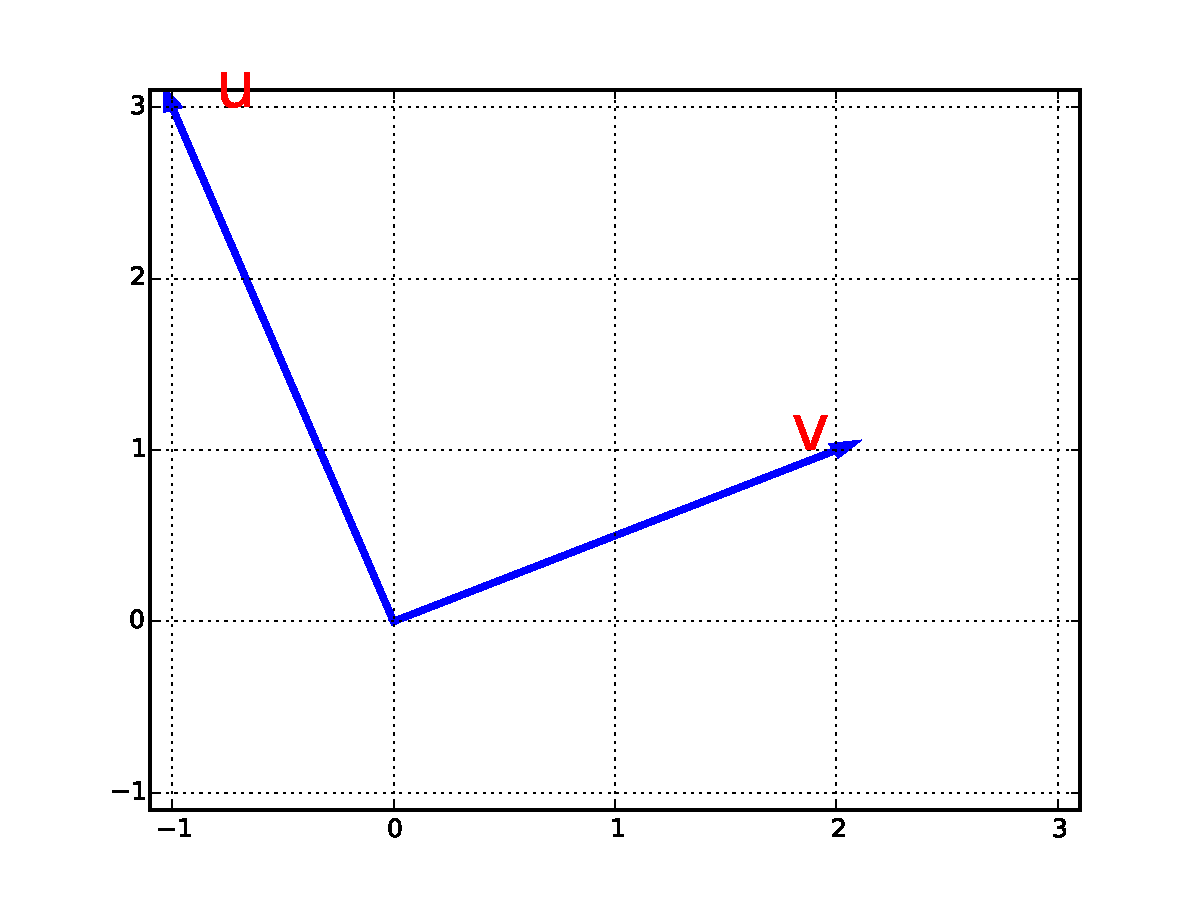
\includegraphics[width=\linewidth]{figs/ex2_1_1.pdf}

\begin{verbatim}
u.dot(v) # 1
v.dot(u) # 1
u.dot(u) # 10
v.dot(v) # 5

u.norm()            # sqrt(10)
u.norm()**2         # 10
v.norm()            # sqrt(5)
v.norm()**2         # 5
(u + v).norm()**2   # 17
(u - v).norm()      # sqrt(13)
\end{verbatim}

\subsubsection{Exercise 2.1.3}
% ----------------------------
Evaluate for
$\mathbf{u} = \left[\begin{matrix}-1\\2\\5\\-3\end{matrix}\right]$ and
$\mathbf{v} = \left[\begin{matrix}2\\-3\\-1\\5\end{matrix}\right]$

\begin{verbatim}
u= Matrix(4, 1, (-1, 2, 5, -3))
v= Matrix(4, 1, (2, -3, -1, 5))
\end{verbatim}

\textbf{Dot product}:

\begin{verbatim}
v.dot(u)    # -28
u.dot(v)    # -28  
v.dot(v)    # 39
u.dot(u)    # 39
\end{verbatim}

Note that commutative property hold. NB \textbf{\texttt{u * v}} raises \texttt{\textcolor{red}{ShapeError: Matrices size mismatch.}}

\textbf{Norm} (\emph{symbol}: $\|u\|$, $\|u + v\|$, $\|u\|^2$, etc)

\begin{verbatim}
u.norm()            # sqrt(39)
u.norm()**2         # 39
v.norm()            # sqrt(39)
v.norm()**2         # 39
(u + v).norm()**2   # 22
\end{verbatim}

\textbf{Distance} $d(u, v) = \| u - v \|$

\begin{verbatim}
(u - v).norm() # sqrt(134)
(v - u).norm() # sqrt(134)
\end{verbatim}

\subsubsection{Exercise 2.1.6}
% ----------------------------

Plot and compute for $\mathbf{u} = \left[\begin{matrix}7\\-2\end{matrix}\right]$
and $\mathbf{v} = \left[\begin{matrix}-5\\3\end{matrix}\right]$

$$\|\mathbf{u} + \mathbf{v} \| = \sqrt{5}$$
and
$$d(\mathbf{u}, \mathbf{v}) = \|\mathbf{u} - \mathbf{v} \| = 13$$

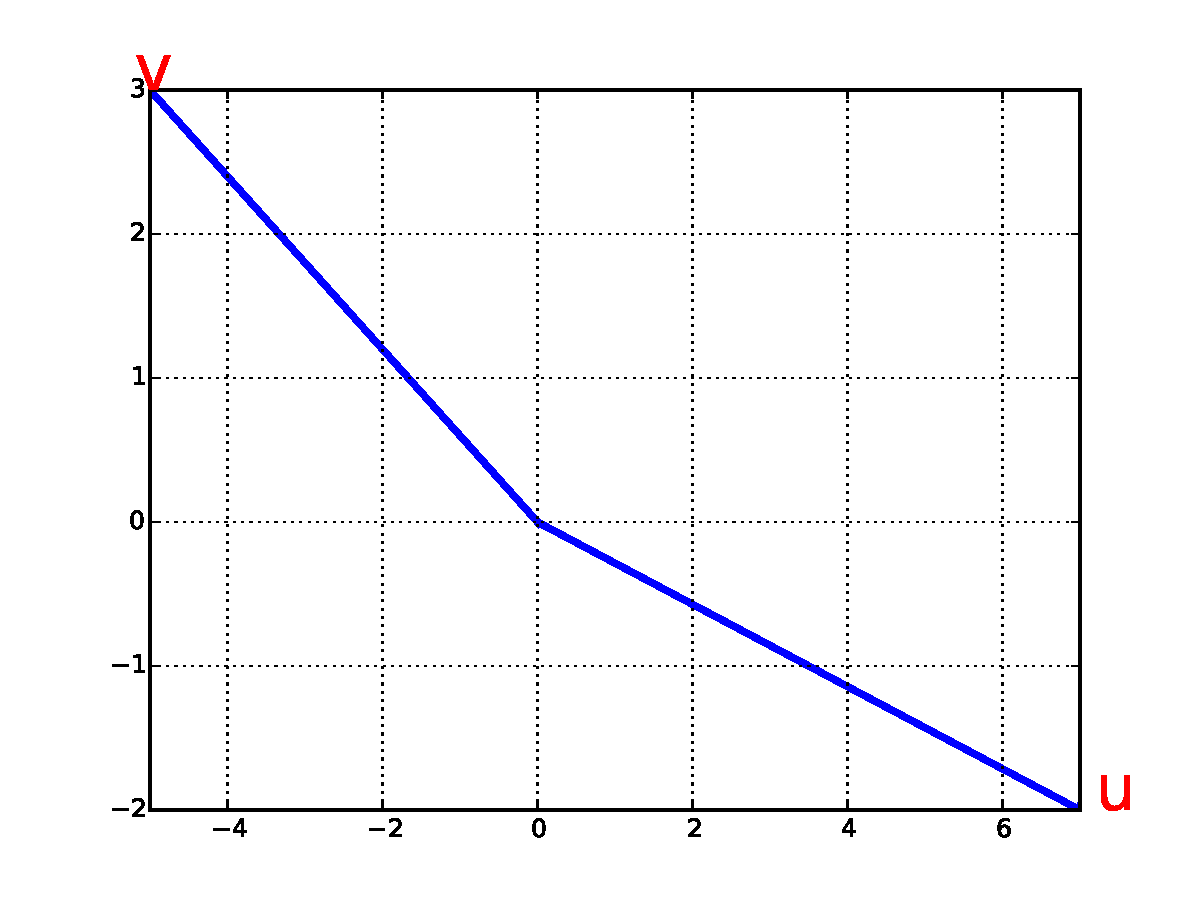
\includegraphics[width=\linewidth]{figs/ex2_1_6.pdf}

\begin{verbatim}
u= Matrix(2, 1, [7, -2])
v= Matrix(2, 1, [-5, 3])

plt.text(float(u[0])+0.2, float(u[1]), 'u', fontsize= 30, color= 'r')
plt.text(float(v[0])-0.2, float(v[1]), 'v', fontsize= 30, color= 'r')
plt.arrow(0, 0, float(u[0]), float(u[1]), lw= 3, color= 'b', head_width=0.05)
plt.arrow(0, 0, float(v[0]), float(v[1]), lw= 3, color= 'b', head_width=0.05)
plt.xlim((-5, 7))
plt.ylim((-2, 3))
plt.grid()
plt.savefig('figs/ex2_1_6.pdf')
plt.close()

(u + v).norm() # sqrt(5)
(u - v).norm() # 13
\end{verbatim}


\subsection{Further Properties of Vectors}
% ========================================

\subsubsection{Exercise 2.2.1}

Find the angle between vectors. The angle is

\begin{equation}\label{eq:uv_angle}
\theta = \arccos(\frac{\mathbf{u} \cdot \mathbf{v}}
{\|\mathbf{u}\| \cdot \|\mathbf{v}\|})
\end{equation}

In \sympy

\begin{verbatim}
def uv_angle(u, v):
    theta= acos(u.dot(v) / (u.norm() * v.norm()))
    return theta
\end{verbatim}

\begin{verbatim}
u= Matrix([1, 1])
v= Matrix([0, 1])
uv_angle(u, v) # pi/4

# As degree:
uv_angle(u, v) * 180/pi # 45

u= Matrix([-1, 2, 3])
v= Matrix([sqrt(2), 1/sqrt(2), -1])
uv_angle(u, v) * 180/pi # ~115 deg
\end{verbatim}

\subsubsection{Exercise 2.2.4}
% ----------------------------
Determine the vector of $k$ so that the vectors are orthogonal to each other.

We want to set the angle between vector equal to 0, \emph{i.e.} Eq. \ref{eq:uv_angle} = 0.

\begin{verbatim}
k= symbols('k', real= True)
u= Matrix([-1, 5, k])
v= Matrix([-3, 2, 7])

eq= Eq(u.dot(v) / (u.norm() * v.norm()) , cos(pi/2))
sol= solve(eq)

# Check
u.subs(k, sol[0]).dot(v) == 0 # True
\end{verbatim}

\subsubsection{Exercise 2.2.6}
% ----------------------------

A vector is normalized by dividing it by its norm. A normalized vector is called
\textbf{unit vector}. In \sympy normlaize with:

\begin{verbatim}
def norm_u(u):
    return u / u.norm()
\end{verbatim}

Determine the value of $k$ so that $\mathbf{\hat{u}} = (1/\sqrt{2}\ 1/2\ k)^T$.

For \textbf{u} to be unit vector, its norm must equal 1. So $\mathbf{\|u\|} = \sqrt{\left\lvert{k}\right\rvert^{2} + 0.75} = 1$.
Solved for $k= \pm 1/2$.

\begin{verbatim}
u= Matrix([1/sqrt(2), 1/2, k])
eq= Eq(u.norm(), 1)
ksol= solve(eq) # [-0.5, 0.5]
\end{verbatim}

\subsubsection{Exercise 2.2.12: Support vector machine}
% -----------------------------------------------------

Find the shortest distance between the vector \textbf{u} and the corresponding
hyperplane. The hyperplane is defined as $\mathbf{v \cdot x} + c = 0$ where
\textbf{v} is a vector of coefficents for the variables in vector \textbf{x} and
$c$ is a constant term. The vector \textbf{u} might represent a data point in
$n$-dimensions.

Remember that an equation in the usual form
$$ax + by +cz + k = 0$$
can be represented in matrix form as
$$ax + by +cz + k
= \left[\begin{matrix}a\\b\\c\end{matrix}\right] \cdot \left[\begin{matrix}x\\y\\z\end{matrix}\right] + k
= \mathbf{v} \cdot \mathbf{x} + k
= 0$$

The shortest distance between \textbf{u} and hyerplane is given by

\begin{equation}\label{eq:ex2_2_12_svm}
d_{shortest} = \frac{|\mathbf{u \cdot v} + c|}{\|\mathbf{v}\|}
\end{equation}

Given \textcolor{red}{$\mathbf{u} = (1\ 1)^T$} and hyperplane \textcolor{blue}{$y= x + 1$}, find the shortes
distance. For this we need to extract the vector of coefficents \textbf{v} from $y= x + 1$, which for convenience can be
re-arranged as $x - y + 1 = 0$.
The coeffients \textbf{v} are $\left[\begin{matrix}1\ \mathit{x} \\ -1\ \mathit{y} \end{matrix}\right]$.

Putting it all together:

\begin{equation}
d_{shortest} = \frac{
    |\left[\begin{matrix}1\\1\end{matrix}\right] \cdot \left[\begin{matrix}1\\-1\end{matrix}\right] + 1|
}{
    \|\left[\begin{matrix}1\\-1\end{matrix}\right]\|
} = \frac{\sqrt{2}}{2} \approx 0.707
\end{equation}

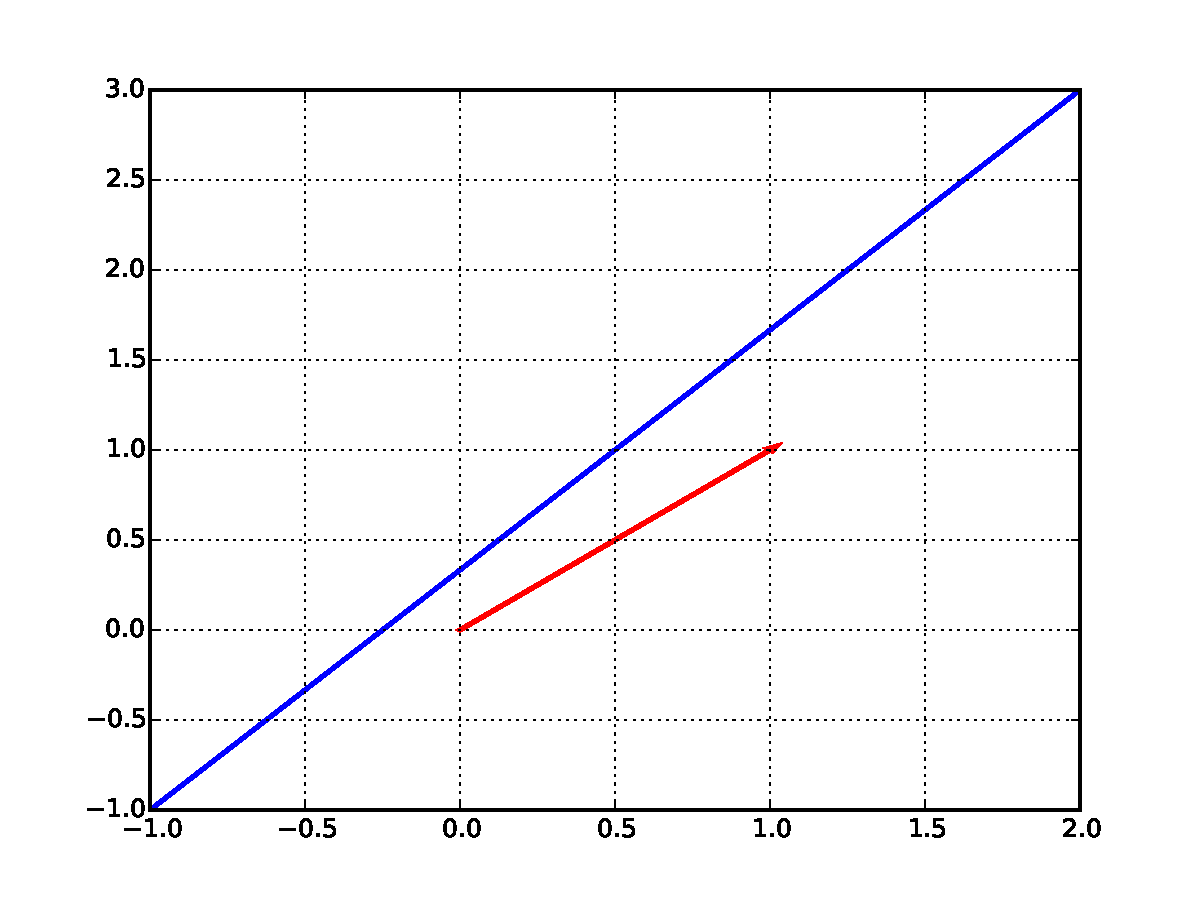
\includegraphics[width=0.75\linewidth]{figs/ex2_2_12_svm.pdf}

\begin{verbatim}
u= Matrix([1, 1])
hyp= Eq(x + 1, y)

# 1. Re-arrange hyp to have x + y + c= 0
hyp2= Eq(hyp.lhs - hyp.rhs)

# 2. Re-arrange in matrix form
cfdict= hyp2.lhs.as_expr().as_coefficients_dict()
v= Matrix([cfdict[x], cfdict[y]])
c= cfdict[numbers.One()]
d_shortest= abs(u.dot(v) + c) / v.norm()
\end{verbatim}

Plotted with:

\begin{verbatim}
plt.plot([-1, 2], [hyp.lhs.subs(x, -2), hyp.lhs.subs(x, 2)], 'b-', lw= 2)
plt.arrow(0, 0, float(u[0]), float(u[1]), lw= 2, color= 'red')
plt.grid()
plt.xlim([-0.5, 1.5])
plt.ylim([-0.5, 1.5])
plt.savefig('figs/ex2_2_12_svm.pdf')
plt.close()
\end{verbatim}

\subsubsection{Exercise 2.2.12d}
% ------------------------------

For $\mathbf{u} = \left[\begin{matrix}1\\2\\3\\4\end{matrix}\right]$ and
$x + 2y + z + w = 10$. We have

$$
d_{shortest}
= \frac{|\mathbf{u} \cdot \mathbf{v} + c|}{\|\mathbf{v}\|}
= \frac{|\left[\begin{matrix}1\\2\\3\\4\end{matrix}\right] \cdot \left[\begin{matrix}1\\2\\1\\1\end{matrix}\right] - 10|}{\|\left[\begin{matrix}1\\2\\1\\1\end{matrix}\right]\|}
= \frac{2 \sqrt{7}}{7}
\approx 0.76
$$

\begin{verbatim}
x,y,z,w = symbols('x y z w')
u = Matrix([1,2,3,4])
hyp= Eq(x + 2*y + z + w, 10)

hyp= hyp.lhs - hyp.rhs
v= [hyp.as_coefficients_dict()[t] for t in (x, y, z, w)]
v= Matrix(v)
c= hyp.as_coefficients_dict()[numbers.One()]

d_shortest= abs(u.dot(v) + c) / v.norm()
\end{verbatim}

\subsection{Linear Independence}
% ==============================

\subsubsection{Exercise 2.3.1}
% ----------------------------

Determine which vectors in $\mathbb{R}^2$ are \textbf{linearly dependent}.

The linear combination of vectors \textbf{u} and \textbf{v} is

\begin{equation}\label{eq:ex2_3_1}
k\mathbf{u} + c\mathbf{v} = \mathbf{O}
\end{equation}

Or more verbose:

\begin{equation}\label{eq:ex2_3_1_II}
k \left[\begin{matrix}x_1\\x_2\end{matrix}\right] +
c \left[\begin{matrix}y_1\\y_2\end{matrix}\right] =
\left[\begin{matrix}0\\0\end{matrix}\right]
\end{equation}

Where $k$ and $c$ are scalars (unknown coefficients). If \ref{eq:ex2_3_1} is
satisfied for $k \neq 0$ or $c \neq 0$ then \textbf{u} and \textbf{v} are
linearly dependent. Which means that \textbf{u} can be expressed as \textbf{v} times
a scalar, or vice versa.

Expressed as a system of equations, \ref{eq:ex2_3_1_II} becomes:

\begin{equation}
\begin{matrix}
kx_1 + cy_1 = 0 \\
kx_2 + cy_2 = 0
\end{matrix}
\end{equation}

Now solve this system and check whether $k=0$ and $c=0$ are the only solutions.

For $\mathbf{u} = \left[\begin{matrix}6\\10\end{matrix}\right]$  and
$\mathbf{v} = \left[\begin{matrix}-3\\-5\end{matrix}\right]$ we have:

$$
k \left[\begin{matrix}6\\10\end{matrix}\right] + c \left[\begin{matrix}-3\\-5\end{matrix}\right] = \left[\begin{matrix}0\\0\end{matrix}\right]
$$

re-arranged as a system

$$
\begin{matrix}6 k - 3 c = 0\\10 k - 5 c = 0\end{matrix}
$$

With solutions $\begin{bmatrix}\begin{Bmatrix}k : \frac{c}{2}\end{Bmatrix}, & \begin{Bmatrix}c : 2 k\end{Bmatrix}\end{bmatrix}$
which hold for $c$ and $k$ different from 0.

\begin{verbatim}
u= Matrix([6, 10])
v= Matrix([-3, -5])
eq1= Eq(k * u[0] + c * v[0], 0)
eq2= Eq(k * u[1] + c * v[1], 0)

csol= solve([eq1, eq2], c)
ksol= solve([eq1, eq2], k)
\end{verbatim}

Note that the conclusion of linear dependence can be reached by looking at the
rank of the matrix $\mathbf{A}= \left[\begin{matrix}\mathbf{u} & \mathbf{v}\end{matrix}\right]$.
In fact, $rank(\mathbf{A})$ is less than 2.

$$
\mathbf{A} = \left[\begin{matrix}\mathbf{u} & \mathbf{v}\end{matrix}\right]
= \left[\begin{matrix}6 & -3\\10 & -5\end{matrix}\right]
$$

with $rank(\mathbf{A}) = 1$. Note that trying to solve \textbf{A} results in
\sympy error \textcolor{red}{\texttt{ValueError: Matrix det == 0; not invertible.}}

In addition, note that the RREF has only one leading row:

$$
\mathbf{A_{rref}} = \begin{pmatrix}\left[\begin{matrix}1 & - \frac{1}{2} & 0\\0 & 0 & 0\end{matrix}\right], & \begin{bmatrix}0\end{bmatrix}\end{pmatrix}
$$

\begin{verbatim}
A= v.col_insert(0, u)
A_rank= A.rank() # 1

try:
    A.solve(Matrix([0, 0])) # Matrix det == 0; not invertible.
except ValueError, e:
    print e
    
A_rref= A.col_insert(2, Matrix([0,0])).rref()
\end{verbatim}

Unit vectors $\mathbf{e_1} = \left[\begin{matrix}1\\0\end{matrix}\right]$ and
$\mathbf{e_2} = \left[\begin{matrix}0\\1\end{matrix}\right]$ are linearly independent.
Note that $rank(\mathbf{A}) = N_{dimensions} = 2$ and the RREF is complete

$$
\mathbf{A_{rref}} = \begin{pmatrix}\left[\begin{matrix}1 & 0 & 0\\0 & 1 & 0\end{matrix}\right], & \begin{bmatrix}0, & 1\end{bmatrix}\end{pmatrix}
$$

\begin{verbatim}
k, c= symbols('k c')
e1= Matrix([1, 0])
e2= Matrix([0, 1])

eq1= Eq(k * e1[0] + c * e1[1], 0)
eq2= Eq(k * e2[0] + c * e2[1], 0)

solve([eq1, eq2]) # {c: 0, k: 0}

# Also
A= e2.col_insert(0, e1)
A_rank= A.rank() # 2

A_rref= A.col_insert(2, Matrix([0,0])).rref()
\end{verbatim}

\subsubsection{Exercise 2.3.12 - \textit{incomplete}}
% ---------------------------------------------------

Determine the value of $t$ in the \textbf{linearly independent} vectors

$$
\mathbf{u} = \left[\begin{matrix}t\\1\\1\end{matrix}\right],
\mathbf{v} = \left[\begin{matrix}-1\\t\\1\end{matrix}\right],
\mathbf{w} = \left[\begin{matrix}1\\1\\t\end{matrix}\right],
$$

The RREF of the augmented matrix is:

$$
\mathbf{A_{rref} = \begin{pmatrix}\left[\begin{matrix}1 & 0 & 0 & 0\\0 & 1 & 0 & 0\\0 & 0 & 1 & 0\end{matrix}\right], & \begin{bmatrix}0, & 1, & 2\end{bmatrix}\end{pmatrix}}
$$

which implies that either the coefficients $k_1 = k_2 = k_3 = 0$ or $t$

\begin{verbatim}
t, k1, k2, k3= symbols('t k1 k2 k3', real= True)

u= Matrix([ t, 1, 1]) # k1
v= Matrix([-1, t, 1]) # k2
w= Matrix([ 1, 1, t]) # k3

eq1= Eq(k1*t - k2   + k3,   0)
eq2= Eq(k1   + k2*t + k3,   0)
eq3= Eq(k1   + k2   + k3*t, 0)

A= w.col_insert(0, v).col_insert(0, u)
Au= Matrix([0,0,0]).col_insert(0, A)
A_rref= Au.rref()
\end{verbatim}

\subsection{Basis and Spanning Set}
% =================================

\subsubsection{Example 2.17}
% ----------------------------

Determine whether the vectors $\mathbf{u} = \left[\begin{matrix}1\\2\end{matrix}\right]$
and $\mathbf{v} = \left[\begin{matrix}-1\\1\end{matrix}\right]$ \textbf{span} $\mathbb{R}^2$.
In other words, the question is whether with the axis \textbf{u} and \textbf{v}
we can draw any vector in $\mathbb{R}^2$. In other words again, can any vector in
$\mathbb{R}^2$ be defined as a \emph{\textbf{linear combination}} of \textbf{u} and \textbf{v}?

So let's take a generic vector in $\mathbb{R}^2$ $\mathbf{w} = \left[\begin{matrix}a\\b\end{matrix}\right]$
and see if the equation

\begin{equation}\label{eq:example_2_17}
\mathbf{w} = k\mathbf{u}  + c\mathbf{v}
\end{equation}

can be solved to find the coefficients \textbf{k} and \textbf{c}.
If the answer is yes, than the generc vector \textbf{w} can be defined in terms
of \textbf{u} and \textbf{v} given appropriate coefficients $k$ and $c$ respectively.

To solve \ref{eq:example_2_17} build the augmented matrix

$$\mathbf{A} =
\left[\begin{matrix}1 & -1 & a\\2 & 1 & b\end{matrix}\right]$$,

put in RREF and see if the RREF is complete. In this case

$$\mathbf{A_{rref}} = \left[\begin{matrix}1 & 0 & \frac{a}{3} + \frac{b}{3}\\0 & 1 & - \frac{2 a}{3} + \frac{b}{3}\end{matrix}\right]$$

The coefficients \textbf{k} and \textbf{c} are given as the last column

\begin{equation}\label{eq:example_2_17_ii}
k, c= \left[\begin{matrix}\frac{a}{3} + \frac{b}{3}\\- \frac{2 a}{3} + \frac{b}{3}\end{matrix}\right]
\end{equation}

Here $a$ and $b$ can be thought as increments on the $x$ and $y$ axis.

For example, how do we express the vector $\mathbf{g} = \left[\begin{matrix}3\\2\end{matrix}\right]$
in the \textbf{spanning set} \textbf{u} and \textbf{v}? By substituting in \ref{eq:example_2_17_ii}
3 for $a$ and 2 for $b$ we get the coefficients $k= 5/3$ and $c = -4/3$. Therefore

\begin{align}
\mathbf{g} = \left[\begin{matrix}3\\2\end{matrix}\right]
= k\mathbf{u} + c\mathbf{v} \\
= \left[\begin{matrix}\frac{a}{3} + \frac{b}{3}\end{matrix}\right] \mathbf{u} + \left[\begin{matrix}- \frac{2 a}{3} + \frac{b}{3} \mathbf{v}\end{matrix}\right] \\
= \left[\begin{matrix}\frac{3}{3} + \frac{2}{3}\end{matrix}\right] \mathbf{u} + \left[\begin{matrix}- \frac{2 \cdot 3}{3} + \frac{2}{3} \mathbf{v}\end{matrix}\right] \\
= 5/3 \mathbf{u} + -4/3 \mathbf{v} \\
= \left[\begin{matrix}3\\2\end{matrix}\right]
\end{align}

\begin{verbatim}
a,b,c,k= symbols('a b c k')

u= Matrix([1, 2])
v= Matrix([-1, 1])
w= Matrix([a, b])

A= w.col_insert(0, v).col_insert(0, u)
A_rref= A.rref()

# Coefficients
k, c= A_rref[0].col(- 1)

# Or maybe easier using M.solve(const)
A= v.col_insert(0, u)
k, c= A.solve(w)

## Represent g in spanning set (u, v)
g= Matrix([3, 2])
k2= k.subs({a:g[0], b:g[1]})
c2= c.subs({a:g[0], b:g[1]})
g2= k2 * u + c2 * v
\end{verbatim}

\subsubsection{Exercise 2.4.1}
% ----------------------------

Determine whether the following vectors span $\mathbb{R}^2$

\begin{verbatim}
# Generic vector
w= Matrix([a, b])

e1= Matrix([1, 0])
e2= Matrix([0, 1])

A= w.col_insert(0, e2).col_insert(0, e1)
\end{verbatim}

For unit vectors $\mathbf{e_1}$ and $\mathbf{e_2}$ the answer is yes with
coefficient a and b from RREF

$$
\mathbf{A_{rref}} = \left[\begin{matrix}1 & 0 & a\\0 & 1 & b\end{matrix}\right]
$$

These vectors do not form a spanning set as a generic vector \textbf{w} cannot be formed
by linear combination. The augmented matrix cannot be in RREF:

$$
\mathbf{A_{rref}} = \left[\begin{matrix}1 & - \frac{1}{2} & 0\\0 & 0 & 1\end{matrix}\right]
$$

Trying to solve the augmented matrix \textcolor{red}{\texttt{ValueError: Matrix det == 0; not invertible.}}

$$
\mathbf{A} = \left[\begin{matrix}2 & -1 & a\\2 & -1 & b\end{matrix}\right]
$$

Results in 

\begin{verbatim}
u= Matrix([2, 2])
v= Matrix([-1, -1])
A= w.col_insert(0, v).col_insert(0, u)
A.rref() # Not in RREF

# Indeed:
A= v.col_insert(0, u)
A.solve(w) # ValueError: Matrix det == 0; not invertible.
\end{verbatim}

\subsubsection{Exercise 2.4.2}
% ----------------------------

Determine whether the following vectors span $\mathbb{R}^3$

\begin{verbatim}
u= Matrix([1, 2, 1])
v= Matrix([2, 4, 0])
w= Matrix([-2, -2, 3])
\end{verbatim}

So, let's define a generic vector in $\mathbb{R}^3$

\begin{verbatim}
a,b,c= symbols('a b c')
g= Matrix([a, b, c])
\end{verbatim}

and define \textbf{g} as a linear combination of \textbf{u, v, w}
\emph{i.e.}
$$ \mathbf{g}= k\mathbf{u} + j\textbf{v} + l\mathbf{w}$$

Can we solve these linear system to find the unknow $k, j, l$?

To answer, prepare the augmented matrix (not really necessary to prepare it though).
Note the use of \texttt{numpy.hstack} to column-bind vectors. Now try to solve it

\begin{verbatim}
A= Matrix(numpy.hstack((u, v, w, g)))
sol= A[:, :-1].solve(A[:, -1])
\end{verbatim}

The syntax to slice the matrix comes from \href{http://docs.scipy.org/doc/numpy/reference/arrays.indexing.html}{NumPy}:
\textcolor{blue}{\texttt{A[:, :-1]}} means get all rows with ':' (1st index) and all columns
excluding the last one with ':-1'.

Anyway, the solution exists and is

$$
k, j, l= \left[\begin{matrix}3 a - \frac{3 b}{2} + c\\- 2 a + \frac{5 b}{4} - \frac{c}{2}\\- a + \frac{b}{2}\end{matrix}\right]
$$

so \textbf{u, v, w} are spanning set of $\mathbb{R}^3$

\subsubsection{Exercise 2.4.3}
% ----------------------------

Determine whether the following vectors form a \textbf{\textit{basis}} for $\mathbb{R}^2$

\begin{verbatim}
u= Matrix([1, 2])
v= Matrix([0, 1])
\end{verbatim}

A \textbf{\textit{basis}} is a spanning set whose vectors are also linearly independent.
This means that a basis is the minimal set of vectors necessary to describe the
$\mathbb{R}^n$ space. Note that if the vectors span $\mathbb{R}^n$ than they are
linearly independent and \emph{vice versa}. So we need to check only one of the two
conditions.

In the case above we have linearl independence since:

$$
A = \left[\begin{matrix}u\\v\end{matrix}\right]
= \left[\begin{matrix}0 & 1\\1 & 2\end{matrix}\right]
$$

and a solution can be found:

$$
a, b= \left[\begin{matrix}- 2 a + b\\a\end{matrix}\right]
$$

\begin{verbatim}
A= Matrix(numpy.array((u, v)))
sol= A.solve(Matrix([a, b]))
A.rank() == A.rows # True (2)
A.det() != 0 # True
A.rref() 
\end{verbatim}

Note also that $rank(A) = 2$, \emph{i.e.} \textbf{A} is full rank and the RREF
is complete $\left[\begin{matrix}1 & 0\\0 & 1\end{matrix}\right]$

In this case, there is no linear independence and the vectors are not a basis:

\begin{verbatim}
u= Matrix([-2, -4])
v= Matrix([1, 2])
A= Matrix(numpy.array((u, v)))
sol= A.solve(Matrix([a, b]))  ## ValueError: Matrix det == 0; not invertible.
A.rank() == A.rows # False
A.det() == 0 # True
\end{verbatim}

\subsubsection{Exercise 2.4.4}
% ----------------------------

Do these vector form a basis for $\mathbb{R}^4$?

\begin{verbatim}
u= Matrix([1, 1, 1, 1])
v= Matrix([1, 1, 0, -1])
w= Matrix([-1, -2, -3, 4])
x= Matrix([2, 2, 2, 2])
A= Matrix(numpy.hstack([u, v, w, x]))
\end{verbatim}

No since they are not linearly independent. In fact u and x are multiple of each other.

\subsubsection{Exercise 2.4.5}
% ----------------------------

Is \textbf{b} in the space spanned by the columns of matrix \textbf{A}?

\begin{equation}
\mathbf{A} = \left[\begin{matrix}1 & 1 & 0\\2 & 5 & 0\\3 & 4 & 9\end{matrix}\right];
\mathbf{b} = \left[\begin{matrix}1\\3\\4\end{matrix}\right]
\end{equation}

To answer we want to know whether the columns of \textbf{A} can be linearly combined
to produce \textbf{b}. Can we found a vector \textbf{k} of coefficients for the
columns in \textbf{A} that produce \textbf{b}?
So we want ot see if we can solve $\mathbf{Ak} = \mathbf{b}$ \emph{w.r.t.} \textbf{k}.
\emph{I.e.} let's try to solve $\mathbf{k}= \mathbf{A}^{-1}\mathbf{b}$. We can solve it
for $\mathbf{k} = \left[\begin{matrix}\frac{2}{3}\\\frac{1}{3}\\\frac{2}{27}\end{matrix}\right]$.

We can also verify that $\mathbf{Ak} = \mathbf{b}$.

\begin{verbatim}
A= Matrix([[1, 1, 0], [2, 5, 0], [3, 4, 9]])
b= Matrix([1, 3, 4])

k= A.inv().dot(b)
# The same:
k= A.solve(b)

# Check back:
b == Matrix(A.dot(k))
\end{verbatim}

What about this case:

\begin{verbatim}
A= Matrix([[1, 2, 3],
           [4, 5, 6],
           [7, 8, 9]])
b= Matrix([1, 3, 4])
A.inv() ## ValueError: Matrix det == 0; not invertible.
A.solve(b) ## The same
\end{verbatim}

\texttt{ValueError: Matrix det == 0; not invertible}, in fact the columns of \textbf{A}
are not linearly independent we cannot find a vector of coefficients \textbf{k} 
to represent \textbf{b}.

\begin{verbatim}
\end{verbatim}

\subsubsection{Exercise 2.4.6}
% ----------------------------

Are these vectors a basis for $mathbb{R}^3$?

\begin{verbatim}
u= Matrix([5, 0, 0])
v= Matrix([0, 6, 0])
w= Matrix([0, 0, 7])
A= Matrix(numpy.hstack([u, v, w]))
A.solve(Matrix([a, b, c])) ## Solvable -> lin. indep. -> basis
\end{verbatim}

What about:

\begin{verbatim}
alpha, beta, lamda= symbols('alpha beta lamda', real= True, nonzero= True)
u= Matrix([alpha, 0, 0])
v= Matrix([0, beta, 0])
w= Matrix([0, 0, lamda])
A= Matrix(numpy.hstack([u, v, w]))
A.solve(Matrix([a, b, c])) ## Solvable -> lin. indep. -> basis

# Also:
A.inv() # Ok
A.rank() == 3 # True
A.det() != 0 # True
\end{verbatim}



\end{document}
